%%%%%%%%%%%%%%%%%%%%%%%%%%%
% PREAMBOLO DEL DOCUMENTO %
%%%%%%%%%%%%%%%%%%%%%%%%%%%
\documentclass[a4paper,11pt,oneside,top=3cm,bottom=3cm,left=3.5cm,right=3.5cm,openright,reqno,table]{book}

% openany - fa iniziare i capitoli direttamente nella pagina successiva
% openright - fa iniziare i capitoli nella prima pagina destra disponibile 
% fleqn  - allinea le formule a sinistra anzichè centrarle
% leqno - dispone la numerazione delle formule sulla sinistra o destra
% reqno - dispone la numerazione delle formule sulla destra
%
\usepackage{packages}
% Per non appesantire troppo questo file
% quasi tutti i pacchetti usati sono salvati in packages.sty
%
\linespread{1.5}
% Per avere la parola BOZZA scritta su tutte le pagine

% funziona solo in modalità PS
% Invece per i PDF ho risolto così:
% pdftk tesi.pdf background bozza.pdf output tesi_bozza.pdf
%
%%%%%%%%%%%%%%%%%%%%%%%%%%%%%%%%%
%   DOCUMENTO VERO E PROPRIO    %
%%%%%%%%%%%%%%%%%%%%%%%%%%%%%%%%%
\begin{document}
% FRONTESPIZIO %
\begin{titlepage}
\changepage{}{}{}{-7.5 mm}{}{}{}{}{}

\begin{center}

\includegraphics [width=.15\columnwidth, angle=0]{unisa}\\ % height
\vspace{0.5cm}
{\LARGE \scshape Università degli Studi di Salerno}\\
\vspace{0.5cm}
{\Large Dipartimento di Informatica}\\
\vspace{0.1cm}
{\large Corso di Laurea Triennale in Informatica}\\
\vspace{1.5cm}
{\Large \scshape Tesi di Laurea} \\
\vspace{4cm}
{\Huge \bfseries Code4Code: tecniche di Intelligenza Artificiale per il suggerimento di Tecnologie Software} \\
\vspace{5cm}

\begin{minipage}[t]{7cm}
\flushleft
\textsc{Relatore}

Prof. \textbf{Fabio Palomba} \\
{\small Università degli studi di Salerno} \\[0.25cm]
\end{minipage}
\hfill
\begin{minipage}[t]{7cm}
\flushright
\textsc{Candidato}

\textbf{Vincenzo Emanuele Martone} \\
Matricola: 0512105758
\end{minipage}

\vspace{2cm}

{\small Anno Accademico 2020-2021}
\end{center}

\end{titlepage}
%

\frontmatter
% quello che segue è in numerazione romana e i capitoli non verranno numerati
% se non si vuole che compaia il numero di pagina basta usare il comando:
%\nonumber

% RINGRAZIAMENTI %
\begin{titlepage}

\nonumber
\null \vspace {\stretch{1}}
	\begin{flushright}
%	\begin{verse}
\textit{"Perché il miglior risultato si ottiene quando ogni componente del gruppo farà ciò che è meglio per sé... e per il gruppo..."\\- John Nash} \\[5mm]
%	\end{verse}
	\end{flushright}



\end{titlepage}
% SOMMARIO %
\cleardoublepage
%\selectlanguage{italian}
\begin{abstract}
Il contesto applicativo della tesi è incentrato sullo studio e sull'applicazione di metodologie di Intelligenza Artificiale nell'ambito di una piattaforma di collaborazione. L'obiettivo principale della tesi sviluppata è quello di fornire un insieme di strumenti di Intelligenza Artificiale da integrare in un'ipotetica piattaforma di collaborazione. Lo scopo di tale piattaforma è quello di mettere in contatto persone intenzionate ad imparare nuove tecnologie in ambito informatico, in modo che possano iniziare una collaborazione che consiste nello scambio di conoscenze relative alle tecnologie che desiderano apprendere. Lo sviluppo della tesi non si concentra sulla creazione della piattaforma completa, bensì sullo studio, sul confronto, sulla progettazione e sull'implementazione di algoritmi di Intelligenza Artificiale che possano assistere gli utenti nell'utilizzo della piattaforma stessa. La tesi fornisce, dunque, un prototipo denominato \textsc{Code4Code} che mostra il funzionamento degli agenti di Intelligenza Artificiale sviluppati. Il problema principale che è stato risolto mediante l'utilizzo dell'Intelligenza Artificiale è quello relativo al suggerimento di tecnologie da imparare sulla base di quelle già conosciute dall'utente; a tale scopo all'utente vengono consigliate sia tecnologie simili a quelle che già conosce, sia tecnologie spesso utilizzate con quelle che già conosce.
\\[1cm]
\end{abstract} 
% INDICI %
\phantomsection
\addcontentsline{toc}{chapter}{Indice}
\tableofcontents
% Il simbolo * serve per evitare che comapaia nell'indice
\clearpage
%\listoffigures
%\clearpage
%\listoftables
% GLOSSARIO
%\cleardoublepage
\phantomsection
\addcontentsline{toc}{chapter}{Glossario}
% per inserire l'elenco dei simboli e degli acronimi nell'indice
\printglossary
% Per stampare il glossario
% per aggiornarlo si deve eseguire da terminale:
% makeindex -s myDoc.ist -t myDoc.alg -o myDoc.acr myDoc.acn
% per inserire una voce nell'elenco:
% \newglossaryentry{voce_etichetta}{name={voce}, description={descrizione}}
% se non compare direttamente nel testo va inizializzata con:
% \glsadd{voce_etichetta}
% oppure se viene richiamata all'interno del testo:
% \gls{voce_etichetta}
% SIMBOLI E NOTAZIONI %
\cleardoublepage
\phantomsection
\addcontentsline{toc}{chapter}{Elenco delle figure}
% per inserire l'elenco dei simboli e degli acronimi nell'indice
%\printglossary[type=\acronymtype,title=Elenco delle figure]
% Per stampare l'elenco dei simboli
\listoffigures
\cleardoublepage
\phantomsection
\addcontentsline{toc}{chapter}{Elenco delle tabelle}
% per inserire l'elenco dei simboli e degli acronimi nell'indice
%\printglossary[type=\acronymtype,title=Elenco delle figure]
% Per stampare l'elenco dei simboli
\listoftables
% per aggiornarlo si deve eseguire da terminale:
% makeindex -s myDoc.ist -t myDoc.glg -o myDoc.gls myDoc.glo
% per inserire una voce nell'elenco:
% \newglossaryentry{voce_etichetta}{name={voce}, description={descrizione}}
% se non compare direttamente nel testo va inizializzata con:
% \glsadd{voce_etichetta}
% oppure se viene richiamata all'interno del testo:
% \gls{voce_etichetta}
\mainmatter
% quello che segue sarà in numerazione araba e i capitoli verranno numerati
%\part{Studio iniziale}
% CAPITOLI
\phantomsection
%\addcontentsline{toc}{chapter}{Introduzione}
\chapter{Introduzione}
\markboth{Introduzione}{}
% [titolo ridotto se non ci dovesse stare] {titolo completo}

\section{Contesto applicativo} %\label{1sec:scopo}
Il lavoro proposto nell'ambito della presente tesi si inserisce nel contesto applicativo delle piattaforme collaborative ed in particolar modo nell'ambito delle piattaforme che mirano all'acquisizione e al miglioramento delle competenze informatiche degli utenti ad esse iscritti mediante una collaborazione tra gli stessi. I benefici che possono essere ottenuti dalla collaborazione nell'ambito di progetti di qualsiasi tipo sono innumerevoli: si può pensare all'aumento della produttività, alla suddivisione del lavoro, alla possibilità di valutare diverse idee evitando di focalizzarsi solo su un numero ristretto di opzioni, alla crescita personale e a tanti altri vantaggi. Se poi si considera l'ambito dello sviluppo Software, ci si rende conto del fatto che la collaborazione non sia un optional in quanto, al giorno d'oggi, un qualsiasi tipo di progetto Software richiede conoscenze di ambiti molto diversi fra loro, non solo dal punto di vista tecnologico. È certamente vero che nell'ambito di un progetto Software sono presenti diversi Team che lavorano con tipi di tecnologie tra loro diversi (ad esempio c'è chi si occupa del \emph{DataBase}, chi si occupa del \emph{Front-End}, eccetera), ma è altrettanto vero che la differenza tra le persone coinvolte in un progetto Software risiede anche nel settore in cui sono specializzate, che non sempre è quello informatico. Dunque, anche se si volessero ignorare i vantaggi derivanti dalla collaborazione che riguardano la produttività e la suddivisione del lavoro, le competenze che sono richieste al giorno d'oggi per lavorare ad un progetto sono difficilmente conciliabili in un unico individuo in quanto riguardano innumerevoli discipline. Risulta, dunque, di fondamentale importanza maturare un approccio alla collaborazione e soprattutto alla comunicazione in quanto non è scontato che persone aventi background diversi riescano a comunicare in maniera agevole ed efficiente. Collaborare insieme ad altre persone ad un progetto non implica necessariamente riuscire a beneficiare di tutti i vantaggi della collaborazione: ci sono casi in cui scarse capacità di comunicazione hanno contribuito al fallimento di progetti. Una recente ricerca \cite{SourceForge} finalizzata all'analisi delle motivazioni per le quali la piattaforma \emph{SourceForge} è stata abbandonata, ha evidenziato vari problemi derivanti da diversi fattori, tra cui i cosiddetti \emph{community smells} ossia 
\begin{quotation}
"caratteristiche organizzative e socio-tecniche sub-ottimali nell'ambito di una community software che può portare a costi aggiuntivi dovuti a problemi di comunicazione, rage-quitting e così via" (Tradotto)
\cite{CommunitySmells}   
\end{quotation}
sintomo di una forte instabilità dal punto di vista organizzativo e comunicativo. I community smells sono stati solo una delle cause che ha portato problemi alla piattaforma, tuttavia non vanno assolutamente sottovalutati in quanto sono comportamenti più comuni di quanto si possa pensare e possono portare a conseguenze peggiori di quelle previste.\\
Il lavoro di tesi svolto, porta il concetto di collaborazione nell'ambito dell'apprendimento di tecnologie Software; tale iniziativa nasce dalla convinzione che anche in quest'ambito sia possibile sviluppare importanti capacità collaborative e soprattutto comunicative da poter sfruttare nell'ambito di progetti Software. Al fine di contestualizzare il lavoro svolto è stato in parte progettato e sviluppato un prototipo di piattaforma collaborativa, denominato \textsc{Code4Code}, che mette a disposizione degli utenti un insieme di strumenti, tra cui l'Intelligenza Artificiale, che li assiste sia in fase di primo approccio alla piattaforma che in fasi più avanzate.  
\section{Obiettivi e risultati}
Sebbene l'idea iniziale del lavoro si focalizzasse sulla creazione completa della piattaforma \textsc{Code4Code}, nel corso dello sviluppo è stata posta una maggiore attenzione verso gli strumenti di supporto che essa dovrebbe fornire agli utenti che ne usufruiscono, in particolar modo alle tecniche di Intelligenza Artificiale utili a migliorare l'esperienza degli utenti. L'obiettivo finale del lavoro svolto è lo sviluppo di due micro-agenti di Intelligenza Artificiale che compongono un unico macro-agente che consiglia Linguaggi \footnote{Nel corso della trattazione, a scopo esemplificativo, si utilizzerà il termine \emph{Linguaggio} per riferirsi, in generale, alla classe dei Linguaggi formali che comprende Linguaggi di Programmazione, Markup, Scripting, Stylesheet [\dots]}, Frameworks e Librerie da studiare sulla base di quelli conosciuti dall'utente che ne usufruisce. Il primo micro-agente consiglia Linguaggi a partire dai Linguaggi conosciuti dall'utente, mentre il secondo micro-agente si occupa di suggerire Frameworks e Librerie sulla base dei Linguaggi, dei Frameworks e delle Librerie conosciuti dall'utente. La suddivisione del macro-agente in due micro-agenti, nonostante la loro apparente similitudine, è stata dettata dalle differenze tra le tecniche di Intelligenza Artificiale impiegate nella realizzazione dei due micro-agenti: il primo micro-agente, infatti, sfrutta le \emph{Association Rules}, mentre il secondo si serve di tecniche di \emph{Natural Language Processing}. In particolar modo:
\begin{itemize}
    \item Le \emph\textbf{Association Rules} sono state impiegate allo scopo di ricavare, dato un insieme di Linguaggi conosciuti dall'utente, altri Linguaggi spesso utilizzati insieme ad essi nell'ambito di progetti Software, mediante semplici regole di tipo statistico applicate ai dati prelevati dalle Repositories pubbliche di \emph{GitHub}. Quest'approccio ha lo scopo di consigliare agli utenti Linguaggi spesso utilizzati insieme a quelli che già conosce, in modo da completare la sua formazione.
    \item Il \emph\textbf{Natural Language Processing} è stato impiegato allo scopo di analizzare un insieme di descrizioni di Frameworks e Librerie ed un insieme di tag di Repositories prelevate da \emph{GitHub} per comprendere la correlazione esistente tra i Frameworks e le Librerie attualmente in voga. Tale analisi consente di stabilire, a partire da un insieme di Linguaggi, Frameworks e Librerie conosciuti da un utente, quali siano i Frameworks e le Librerie da consigliargli. 
\end{itemize}
L'utilizzo dell'Intelligenza Artificiale verrà debitamente trattato ed approfondito nel corso dei successivi capitoli.\\Dopo aver esaminato il dominio del problema e stabilito quali tecniche di Intelligenza Artificiale utilizzare, sono stati studiati i fondamenti teorici di tali tecniche che hanno reso possibile, in fase implementativa, un utilizzo consapevole delle Librerie adoperate per la creazione degli Agenti Intelligenti di interesse. Durante la fase implementativa ci si è prima di tutto soffermati sulla creazione dei singoli micro-agenti, successivamente è stato effettuato un lavoro di integrazione tra i micro-agenti stessi ed infine è stata aggiunta un'interfaccia utente per rendere possibile un utilizzo agevole di quanto implementato. La fase implementativa ha richiesto numerose revisioni del DataSet e dei parametri di addestramento dei micro-agenti fino al raggiungimento di un risultato che, rapportato alle caratteristiche dei DataSet in esame e alla conoscenza dell'ambito delle attuali tecnologie Software utilizzate, fosse intuitivamente sensato e contenesse il minor numero possibile di \emph{outliers}. Il risultato finale di tale lavoro di tesi risulta, dunque, essere un prototipo della piattaforma Web \textsc{Code4Code} tramite il quale si può interagire con l'Intelligenza Artificiale sviluppata.  
\section{Struttura della tesi}
La trattazione del lavoro di tesi verrà suddivisa in cinque capitoli di cui viene data, di seguito, una breve descrizione:
\begin{itemize}
    \item Il Primo Capitolo introduce il contesto applicativo, gli obiettivi e i risultati del lavoro di tesi svolto.
    \item Il Secondo Capitolo analizza le caratteristiche fondamentali di alcune piattaforme collaborative considerate particolarmente rilevanti e affini alla piattaforma \textsc{Code4Code}.
    \item Il Terzo Capitolo rappresenta il cuore della tesi in quanto descrive nel dettaglio le tecniche di Intelligenza Artificiale adoperate motivando le scelte che sono state effettuate a tal proposito.
    \item Il Quarto Capitolo illustra la progettazione e l'architettura della piattaforma Web \textsc{Code4Code} presentando le tecnologie adoperate per l'effettiva creazione del prototipo implementato.
    \item Il Quinto Capitolo conclude la trattazione del lavoro di tesi presentando considerazioni di carattere generale sul lavoro svolto e sugli eventuali sviluppi futuri.
\end{itemize}
\chapter{Piattaforme collaborative e di apprendimento} %\label{1cap:spinta_laterale}
% [titolo ridotto se non ci dovesse stare] {titolo completo}
%
\begin{citazione}
Questo capitolo fa una breve panoramica sulle piattaforme collaborative e di apprendimento considerate affini alla piattaforma \emph{Code4Code}. Tale trattazione fornisce un'idea della motivazione per la quale si è ritenuto utile progettare la piattaforma e soprattutto formulare e risolvere problemi ad essa inerenti.
\end{citazione}
\newpage

\section{Differenza tra piattaforme collaborative e di apprendimento} %\label{1sec:scopo}
I concetti di piattaforma collaborativa e di piattaforma di apprendimento sono ben distinti. Una piattaforma collaborativa è, in generale, un tipo di piattaforma in cui gli utenti collaborano tra loro al fine di raggiungere uno scopo comune, mentre una piattaforma di apprendimento è un tipo di piattaforma che mira ad accrescere le conoscenze e le competenze di chi ne usufruisce. La natura del secondo tipo di piattaforma non è intrinsecamente legata ad un approccio basato sulla cooperazione tra gli utenti che vi partecipano, infatti nella maggior parte dei casi l'apprendimento risulta essere unidirezionale da insegnante ad allievo. Nell'ambito delle piattaforme di apprendimento vengono, spesso, inserite funzionalità di comunicazione tra allievo ed insegnante al fine di rendere agevole l'apprendimento tramite un confronto grazie al quale l'allievo può esporre i propri dubbi all'insegnante. Nonostante ciò, difficilmente il confronto tra le due parti avviene in tempo reale, e spesso si ricorre ad una sezione dedicata alle domande degli allievi a cui l'insegnante può rispondere in differita. Una piattaforma di collaborazione, d'altro canto, non è necessariamente legata all'apprendimento ma generalmente fornisce un insieme di strumenti per facilitare la comunicazione e la collaborazione in tempo reale.  
\section{Esempi di piattaforme collaborative}
Al giorno d'oggi esistono diverse piattaforme collaborative che consentono a chi ne usufruisce di collaborare insieme ad altri utenti per raggiungere uno scopo comune. Di seguito verranno elencate alcune piattaforme e ne verranno brevemente analizzate le caratteristiche fondamentali.
\begin{itemize}
    \item{\textbf{GitHub}: oltre a fungere da hosting per i progetti software degli utenti che ne usufruiscono, fornisce strumenti per la gestione del \emph{Version Control} che risulta essere di fondamentale importanza soprattutto nel caso di progetti di gruppo in cui gli sviluppatori devono collaborare tra loro.}
    \item{\textbf{Slack}: progettata per la collaborazione aziendale, fornisce un insieme di strumenti utili alla comunicazione istantanea tra gli utenti stessi. In particolare grazie a Slack è possibile avviare chiamate e videochiamate con funzionalità di condivisione schermo, usufruire di una chat in tempo reale e condividere file grazie all'integrazione con alcune piattaforme di condivisione come ad esempio \emph{Google Drive, Dropbox e Microsoft OneDrive}.}
\end{itemize}
\section{Esempi di piattaforme di apprendimento}
La progettazione di una piattaforma di apprendimento è un lavoro che determina in gran parte l'efficacia dell'apprendimento degli utenti che ne usufruiscono. Di seguito verranno esaminate alcune piattaforme con i relativi approcci alla progettazione dell'apprendimento.
\begin{itemize}    
    \item{\textbf{MasterClass}: mediante il pagamento di un abbonamento, consente agli utenti di accedere ad un insieme di corsi che abbracciano diversi ambiti, tra cui il business, la musica, la scrittura e la tecnologia. I corsi sono tenuti da esperti del settore, grazie ai quali la qualità dei corsi risulta essere elevata, tuttavia la piattaforma non garantisce un'interazione tra studenti ed insegnanti, sebbene non manchino alcune occasioni in cui gli studenti possono sottoporre il proprio lavoro ad una revisione da parte degli insegnanti.}
    \item{\textbf{Udemy}: consente agli utenti di usufruire di corsi (sia gratuiti che a pagamento) erogati da altri utenti della piattaforma. Ogni corso è suddiviso in lezioni, in corrispondenza di ognuna delle quali è indicato l'argomento affrontato mediante un breve titolo. È, inoltre, disponibile una sezione Q\&A in cui gli studenti del corso possono porre domande all'insegnate e chiunque può partecipare alla discussione. È disponibile una funzionalità di Messaggi Diretti tra studenti ed insegnanti solo per i corsi a pagamento al fine di ottenere delucidazioni sugli argomenti trattati nei corsi e per dare feedback. Infine gli insegnanti possono pubblicare degli annunci volti alla distribuzione di materiali gratuiti relativi ai loro corsi.}
\end{itemize}
\section{Tandem: una piattaforma che unisce collaborazione ed apprendimento}
La piattaforma \emph{Code4Code} si ispira concettualmente ad una piattaforma che unisce collaborazione ed apprendimento: \textbf{Tandem}. Tandem è un'App sviluppata per Android e iOS che serve a mettere in contatto utenti che vogliono imparare nuove lingue. La piattaforma associa ad un utente che vuole imparare una lingua \emph{A} e conosce una lingua \emph{B} un utente che conosce la lingua \emph{A} e vuole imparare la lingua \emph{B}. I due utenti, una volta in contatto, possono dialogare effettuando un lavoro di mutua correzione, senza instaurare un rapporto insegnante-studente. Tale approccio è detto \emph{Tandem Language Learning} \cite{tandem} ed è il principio cardine della piattaforma \emph{Code4Code}.\\Tandem fornisce come strumenti di supporto per la comunicazione chiamate, videochiamate e chat in tempo reale, in cui è possibile anche inviare messaggi vocali (fondamentali per esercitare la pronuncia della lingua). 
\section{Considerazioni sulle piattaforme analizzate}
Dalla breve analisi effettuata, risulta evidente che in molti casi ci sia un compromesso tra qualità dei corsi erogati ed interazione con gli insegnanti. L'approccio utilizzato da \emph{Tandem} fa emergere, in maniera evidente, tale compromesso, in quanto il generico interlocutore potrebbe non avere un background educazionale, per cui l'esperienza dal punto di vista pratico potrebbe risultare meno scorrevole di un'esperienza di insegnamento tradizionale come quella proposta da alcune delle piattaforme sopracitate in cui si partecipa a corsi pre-registrati. La problematica appena trattata rappresenta uno degli aspetti critici del metodo \emph{Tandem Language Learning}. D'altro canto tale approccio favorisce al massimo l'interazione tra le parti che vogliono apprendere e non rende necessario il pagamento di una somma di denaro, in quanto la moneta di scambio per la conoscenza è la conoscenza stessa. La piattaforma \emph{Code4Code} propone un tipo di approccio all'apprendimento basato sulla collaborazione: se un utente \emph{X} conosce la Tecnologia \emph{A} e vuole studiare la Tecnologia \emph{B}, mentre un utente \emph{Y} conosce la Tecnologia \emph{B} e vuole studiare la Tecnologia \emph{A}, potranno mettersi in contatto e, tramite la piattaforma, scambiarsi conoscenze relative alle Tecnologie mediante lezioni in tempo reale tenute dagli utenti stessi, chat ed esercizi. 
\chapter{Background sull'Intelligenza Artificiale utilizzata} %\label{1cap:spinta_laterale}
% [titolo ridotto se non ci dovesse stare] {titolo completo}
%

\begin{citazione}
Come anticipato nei precedenti capitoli, è stata posta particolare attenzione alla progettazione e all'implementazione degli strumenti di Intelligenza Artificiale che assistono gli utenti nell'utilizzo della piattaforma. Il presente capitolo risulta, dunque, essere il cuore del lavoro di Tesi in quanto tratta e approfondisce diversi aspetti relativi all'Intelligenza Artificiale. 
\end{citazione}
\newpage

\section{Motivazioni all'utilizzo dell'Intelligenza Artificiale} %\label{1sec:scopo}
L'utilizzo dell'Intelligenza Artificiale apre le porte all'implementazione di funzionalità che arricchiscono la piattaforma all'interno della quale vengono integrate. Nel caso della piattaforma \emph{Code4Code} ci sono due motivazioni principali che portano all'esigenza di utilizzare l'Intelligenza Artificiale:
\begin{itemize}
    \item{\textbf{Suggerimento di Tecnologie Software}: Quando un utente si iscrive alla piattaforma potrebbe non avere le idee chiare sulle Tecnologie da apprendere: un apposito modulo di Intelligenza Artificiale lo assisterà consigliandogli Tecnologie da imparare sulla base di quelle che già conosce.}
    \item{\textbf{Suggerimento di utenti con cui collaborare}: L'anima della piattaforma è la collaborazione, ma la disponibilità di un utente può variare in base a diversi fattori come il numero di utenti con cui collabora in un certo momento. Mediante un algoritmo di Intelligenza Artificiale è possibile individuare un insieme di utenti con cui risulta più conveniente iniziare una collaborazione evitando lunghe ed inconcludenti ricerche nel momento in cui si è in procinto di iniziare una collaborazione.}
\end{itemize}
Tra queste due problematiche è stata debitamente affrontata, progettata ed implementata solo la prima, mentre della seconda verrà fornita solo un'idea di progettazione ed implementazione.
\section{Suggerimento di Tecnologie Software} %\label{1sec:scopo}
Quando un utente si iscrive alla piattaforma seleziona le Tecnologie Software conosciute, sulla base delle quali gliene vengono suggerite altre da imparare. Una Tecnologia Software, in questo specifico caso, può essere un Linguaggio \footnote{Nel corso della trattazione, a scopo esemplificativo, si utilizzerà il termine \emph{Linguaggio} per riferirsi, in generale, alla classe dei Linguaggi formali che comprende Linguaggi di Programmazione, Markup, Scripting, Stylesheet [\dots]}, un Framework o una Libreria, pertanto il problema in questione è stato suddiviso in due parti: 
\begin{itemize}
    \item Suggerimento di Linguaggi a partire da quelli conosciuti, mediante \emph{Association Rules}.
    \item Suggerimento di Librerie e Frameworks a partire dai Linguaggi, dalle Librerie e dai Frameworks conosciuti, mediante \emph{Natural Language Processing}. 
\end{itemize}
L'esigenza di suddividere l'Agente di Intelligenza Artificiale in due micro-agenti è stata dettata dalla eterogeneità dei DataSet disponibili a causa dei quali non è stato possibile pensare ad una soluzione unificata per risolvere il problema. Nei paragrafi successivi verranno trattati gli aspetti teorici ed implementativi delle tecniche di Intelligenza Artificiale utilizzate con riferimenti ai relativi DataSet.
\subsection{Suggerimento di Linguaggi}
Suggerire un Linguaggio di Programmazione ad un utente in base a quelli che conosce, significa proporre all'utente Linguaggi che siano in qualche modo correlati a quelli di sua conoscenza. È sensato considerare due principali tipi di correlazione: \emph{similarità} e \emph{complementarietà}.
\begin{itemize}
    \item Due Linguaggi vengono considerati simili se hanno un certo numero di caratteristiche in comune.
    \item Due Linguaggi vengono considerati complementari se vengono spesso utilizzati insieme nell'ambito di Progetti Software.
\end{itemize}
\subsubsection{Similarità tra Linguaggi}
Stabiliti i parametri secondo i quali due Linguaggi sono definibili simili, risulta semplice sviluppare un Algoritmo che, presi in input i Linguaggi conosciuti dall'utente, restituisca quelli che hanno più caratteristiche possibili in comune con i Linguaggi input. Le caratteristiche in esame sono: tipo del Linguaggio (Programmazione, Markup, Scripting, Query, Stylesheet [\dots]), paradigmi (Object Oriented, funzionale, procedurale [\dots]) e sistema di tipizzazione (nessuna tipizzazione, tipizzazione forte, tipizzazione debole). 
Supponendo, ad esempio, che il Linguaggio input sia \emph{Java} che è un Linguaggio di Programmazione, il cui paradigma è \emph{Object Oriented}, con sistema di tipizzazione forte, l'Algoritmo suggerirà sicuramente \emph{Kotlin} (le cui caratteristiche corrispondono quasi esattamente a quelle di \emph{Java}) in misura maggiore rispetto ad un Linguaggio di Markup come ad esempio \emph{HTML} o ad un Linguaggio di Scripting come ad esempio \emph{Lua}. 
La metrica adottata per quantificare quanto un Linguaggio sia effettivamente consigliato ad un utente è esattamente il numero di caratteristiche che il Linguaggio input e gli altri Linguaggi hanno in comune. 
L'Algoritmo non restituisce un unico Linguaggio, bensì un insieme di Linguaggi aventi un certo numero di caratteristiche in comune con almeno uno dei Linguaggi input. Il numero massimo di Linguaggi da consigliare all'utente è stato scelto in seguito ad alcuni test per individuare la soluzione migliore: se la dimensione \emph{n} dell'insieme dei Linguaggi restituiti dall'Algoritmo supera le 5 unità, si considerano solo i primi \(\frac{n}{2}\) Linguaggi più simili, in caso contrario si considerano tutti i Linguaggi restituiti. \\
Dal momento che i dati da esaminare riguardano le caratteristiche dei vari Linguaggi, è stato ottenuto un semplice DataSet prelevando i dati da siti Web come \emph{Wikipedia}. L'Algoritmo vero e proprio è stato sviluppato in \emph{Java} senza l'ausilio di particolari Framework o Librerie. \\
L'approccio appena descritto non rappresenta una vera e propria applicazione di Intelligenza Artificiale, ma solo una base esemplificativa da cui partire per poter stabilire, in maniera intuitiva, la similarità tra due Linguaggi. L'approccio basato sulla complementarietà, descritto di seguito, costituisce un esempio di applicazione dell'Intelligenza Artificiale sicuramente più articolato rispetto a quello appena presentato.
\subsubsection{Complementarietà tra Linguaggi}
Focalizzarsi sulla complementarietà tra i Linguaggi consente, a chi vuole imparare, di acquisire competenze a 360 gradi.
 Come anticipato in precedenza, due Linguaggi sono considerati complementari se vengono spesso utilizzati insieme nell'ambito di Progetti Software; per indagare sulla complementarietà tra i Linguaggi, è necessario disporre sia di un insieme di Progetti Software di dimensione sufficientemente elevata, al fine di poter effettuare considerazioni reali sull'associazione tra i Linguaggi, che di una tecnica per interpretare e dare un senso ai dati relativi ai progetti. Al fine di ottenere un insieme considerevole di Progetti Software è stato utilizzato \emph{GitHub} ed in particolar modo è stato fatto riferimento alle Repositories pubbliche.
\emph{GitHub} mette a disposizione API pubbliche e gratuite che assolvono a diversi scopi, tra cui cercare i progetti ed ottenere informazioni relative ad essi. Tuttavia, per semplificare il lavoro e migliorare la qualità del DataSet è stato utilizzato un tool online denominato \emph{SEART GitHub Search Engine} \cite{Dabic:msr2021data} che consente, mediante un'interfaccia molto intuitiva, di filtrare i risultati secondo determinate caratteristiche della Repository come: numero di commits, numero di stars, numero di releases, range di data. 
Effettuare un filtraggio del genere consente di evitare Repositories non rilevanti (Repositories di prova, piccoli progetti di esempio, esercizi didattici) focalizzando l'attenzione solo su quelle che possano in qualche modo essere rilevanti ai fini della trattazione del problema in questione. 
I parametri utilizzati per filtrare le Repositories sono stati scelti in maniera intuitiva e sono stati effettuati dei test per confrontarli tra loro. Il risultato migliore è stato ottenuto prelevando tutte le Repositories con almeno 50 commit e 100 stars. Il Tool sopracitato ha prodotto un file output in formato \emph{JSON}, del quale è stato effettuato un parsing utilizzando uno script scritto in \emph{Python} tramite il quale sono state estratte le informazioni rilevanti per la risoluzione del problema in questione, ossia i Linguaggi impiegati nell'ambito delle Repositories con la relativa quantità di byte di codice utilizzato. È stato, dunque, creato un file in cui su ogni riga è riportata la lista di Linguaggi utilizzati in una determinata Repository, ciascuno dei quali è seguito dalla quantità di byte di codice scritto in quel Linguaggio. Ogni riga è, dunque, associata ad una specifica Repository ed in totale sono stati estratti i dati relativi a esattamente 51135 Repositories. \\
Il file appena descritto funge da DataSet per l'Algoritmo che cerca la correlazione tra i Linguaggi basandosi sulla complementarietà tra gli stessi. 
I dati vengono interpretati mediante le \emph{Association Rules} \cite{AssociationRules}, un metodo che serve ad estrarre relazioni nascoste da una grande quantità di dati. Nel caso in esame, la relazione da ricercare nei dati è la presenza simultanea di Linguaggi nella stessa Repository; le Association Rules fanno proprio questo tipo di lavoro considerando tre misure di probabilità denominate \emph{Support, Confidence e Lift}.
\begin{itemize}
    \item Il \textbf{Support} è una misura che indica la frequenza in cui un determinato Linguaggio compare nei dati in esame. Il Support di un linguaggio L in un DataSet contenente N Repositories si calcola nel seguente modo: 
        \begin{equation}    
            Support(L)=\frac{Freq(L)}{N}
        \end{equation}    
    \item La \textbf{Confidence} è una misura che indica la frequenza con cui un Linguaggio L\textsubscript2 è presente nelle Repositories che contengono un Linguaggio L\textsubscript1. La formula per calcolare la Confidence è la seguente:
        \begin{equation}
            Confidence(L_1 \rightarrow L_2)=\frac{Support(L_1 \cap L_2)}{Support(L_1)}
        \end{equation}
    \item Il \textbf{Lift} è una misura simile alla \emph{Confidence}, in quanto indica la frequenza con cui un Linguaggio L\textsubscript2 è presente nelle Repositories che contengono un Linguaggio L\textsubscript1, tuttavia tiene conto anche della popolarità del Linguaggio L\textsubscript2. Dal punto di vista matematico, si calcola nel seguente modo:
        \begin{equation}
            Lift(L_2)=\frac{Support(L_1 \cap L_2)}{Support(L_1) \times Support(L_2)}
        \end{equation}
\end{itemize}
L'algoritmo Apriori sfrutta queste tre misure di probabilità al fine di generare le Association Rules. Tralasciando i dettagli implementativi dell'Algoritmo Aprori (che possono essere approfonditi alla fonte indicata \cite{AssociationRules}), se si considera un sottoinsieme di k Linguaggi del DataSet sarà possibile generare $2^k-2$ Association Rules, ciascuna delle quali avrà la seguente forma:
\begin{equation}
    \{L_1, L_2, \dots, L_i\} \rightarrow \{L_{i+1}, \dots, L_k\}
\end{equation}
Ad ogni Association Rule sono associate la Confidence e il Lift relativi ai Linguaggi $\{L_{i+1}, \dots, L_k\}$ (tale termine della Regola è detto \emph{conseguente}) considerando le Repository contenenti i Linguaggi $\{L_1, L_2, \dots, L_i\}$ (tale termine della Regola è detto \emph{antecedente}), e ad ogni gruppo di Association Rules relativo ad un sottoinsieme di k Linguaggi è associato il Support dei Linguaggi stessi.
L'Algoritmo Apriori non è stato implementato da zero, ma è stata utilizzata una sua implementazione in Python denominata \emph{Apyori} \cite{Apyori} che consente di eseguire l'algoritmo in maniera agevole a partire dal DataSet di Repositories descritto in precedenza e di impostare i parametri di funzionamento dell'Algoritmo come la soglia di Support, Confidence e Lift minime dei Linguaggi che l'Algoritmo deve considerare e la dimensione massima dei sottoinsiemi che devono essere usati dall'Algoritmo per generare le Association Rules. A tal proposito, i parametri che sono stati scelti riguardano la soglia di Support e Confidence poste rispettivamente a 0.0045 e 0.10.\\
Quanto descritto fino ad adesso non dipende dall'input dell'utente e fa, dunque, parte di un lavoro che viene svolto offline e che funge da base per l'Algoritmo vero e proprio che a partire dai Linguaggi conosciuti dall'utente ne suggerisce altri. Tale Algoritmo, infatti, preleva tutte le Association Rules che come antecedente contengono i Linguaggi input e considera i Linguaggi contenuti nel termine conseguente; la lista di questi Linguaggi verrà chiamata \emph{Lista di Linguaggi candidati}. Ad ogni Linguaggio facente parte della \emph{Lista di Linguaggi candidati}, l'Algoritmo associa la Confidence della Regola a cui appartiene (in caso di Linguaggi duplicati considera quello appartenente alla Regola con Confidence maggiore) e consiglia alcuni di questi Linguaggi agli utenti. Non vengono consigliati tutti i Linguaggi candidati per due motivi principali: 
\begin{itemize}
    \item Il primo motivo riguarda aspetti puramente legati all'usabilità della piattaforma, per cui non si consigliano troppi Linguaggi all'utente per evitare di confonderlo. A tale scopo dopo aver ottenuto la lista dei Linguaggi candidati, l'Algoritmo controlla la sua dimensione \emph{n} e se questa è inferiore o uguale a 10, non scarta alcun Linguaggio, se è compresa tra 10 e 19, conserva solo gli \emph{n/2} Linguaggi a cui è associata la Confidence più elevata, se supera 20 vengono conservati solo gli \emph{n/4} Linguaggi con la Confidence più elevata.
    \item Il secondo motivo riguarda la presenza di Linguaggi nelle Repositories che pur essendo molto frequenti, non risultano rilevanti. Ad esempio, in molti Progetti sono presenti brevi script scritti in Bash utilizzati per motivi riguardanti la configurazione e l'esecuzione del Progetto; non sarebbe, dunque, corretto consigliare Bash unicamente perché molto usato insieme ad un determinato Linguaggio input. 
    Risulta, dunque, necessario svolgere un lavoro di tipo statistico su ogni Linguaggio candidato per determinare se, nelle Repositories in cui viene utilizzato insieme ad almeno uno dei Linguaggi input dell'utente, ha una percentuale di utilizzo almeno pari ad una determinata soglia. La percentuale di utilizzo di un Linguaggio in una Repository può essere facilmente ricavata a partire dalla quantità di byte di codice scritto in quel Linguaggio; ai fini dell'Algoritmo viene effettuata una media delle percentuali di codice scritto nel Linguaggio candidato considerato: verranno scartati tutti i Linguaggi la cui media di percentuale di codice impiegato nelle Repositories risulta essere inferiore al 3.5\% (tale soglia è stata scelta dopo aver effettuato diversi test e confrontato tra loro i risultati). 
\end{itemize}
\subsection{Suggerimento di Frameworks e Librerie: Natural Language Processing}
Suggerire Frameworks e Librerie ad un utente a partire dai Linguaggi, dai Frameworks e dalle Librerie che conosce, si è rivelato essere un lavoro meno agevole del precedente, in quanto le API di GitHub consentono di ricavare i Linguaggi adoperati in una Repository, ma non i Frameworks e le Librerie. È stata, dunque, adottata una tecnica di Intelligenza Artificiale diversa dalla precedente, al fine di sfruttare al meglio il DataSet in possesso; tale DataSet contiene:
\begin{itemize}
    \item Descrizioni in lingua inglese di Linguaggi, Framework e Librerie estratti tramite uno scraper scritto in \emph{JavaScript} dalla pagina di GitHub relativa ai Topic (tra cui Frameworks e Librerie) relativi alle Repositories. 
    \item Lista di Tag relativi a diverse Repositories estratti da GitHub tramite uno scraper appositamente scritto in \emph{JavaScript}. A differenza del caso dei Linguaggi, tuttavia, i tag sono inseriti dagli utenti e non sempre alla stessa Libreria/Framework corrisponde la stessa stringa, in quanto spesso vengono utilizzati nomi alternativi ed abbreviazioni (ciò non accade nel caso dei Linguaggi in quanto vengono automaticamente impostati da GitHub). 
\end{itemize}
Vista l'irregolarità e l'informalità del DataSet in esame, si è deciso di ricorrere a tecniche di \emph{Natural Language Processing} al fine di poter interpretare e dare un senso ai dati ed estrarre informazioni utili sulla correlazione tra i Frameworks, sulla correlazione tra le Librerie e sulla correlazione tra Frameworks e Librerie. L'Algoritmo di NLP utilizzato è \emph{Word2Vec} \cite{Word2Vec} che è basato su una Rete Neurale con un singolo livello nascosto il cui scopo è quello di calcolare un insieme di vettori al fine di valutare la similarità tra le parole facenti parte del DataSet. Quando si parla di \emph{Doc2Vec} è necessario dettagliare il concetto di DataSet mediante termini specifici: in primo luogo l'unità di base del DataSet è il \emph{documento}, definito come testo di qualsiasi tipo (una breve descrizione, un paper, un libro...) e che nel caso in questione risulta essere la descrizione di una Libreria/Framework oppure l'insieme di tag relativi ad una singola Repository. Un insieme di \emph{documenti} forma un \emph{Corpus}, che funge da input per l'Algoritmo e dal quale si estraggono le parole al fine di costruire un dizionario. Come anticipato, l'Algoritmo \emph{Word2Vec} fa uso di una rete neurale, nella quale è possibile individuare:
\begin{itemize}
    \item Un livello input che trasforma le parole in vettori: in primo luogo l'Algoritmo crea un dizionario contenente tutte le \emph{n} parole del \emph{Corpus} e alla parola i-esima associa un vettore di dimensione \emph{$1\times n$} composto da valori tutti pari a 0 e da un 1 in posizione i-esima; tali vettori sono chiamati \emph{one-hot vector}. 
    \item Un livello nascosto che contiene \emph{n} vettori, ciascuno di dimensione \emph{m}; la scelta di \emph{m} è, generalmente, problem specific e rappresenta il numero di \emph{features} delle parole nel dizionario considerato. Lo scopo della fase di addestramento è quello di apprendere i valori delle componenti dei vettori dello strato nascosto della rete, in quanto rappresentano le caratteristiche vere e proprie delle parole del dizionario; tali vettori sono denominati \emph{embeddings} e il livello nascosto della rete contiene una matrice \emph{$n \times m$} di tutti gli \emph{embeddings} relativi alle parole del dizionario.
    \item Un livello output nel quale viene effettuato il prodotto tra l'\emph{embedding} della parola input e la matrice che contiene tutti gli \emph{embeddings} trasposta, e successivamente al risultato viene applicata la funzione di regressione Softmax, ottenendo un vettore contenente la probabilità che ogni parola del dizionario si trovi nel contesto della parola input.
\end{itemize} 
L'addestramento della rete neurale consiste in diverse fasi: in primo luogo vi è la definizione di un valore intero detto \emph{window size} che rappresenta il numero di parole da considerare a sinistra e a destra di una parola \emph{w} all'interno di una frase del \emph{Corpus}. Tali parole saranno considerate appartenenti allo stesso contesto di \emph{w} e sono dette \emph{parole di contesto}. Vengono, a questo punto, costruiti dei campioni di addestramento ossia delle coppie \emph{(w, x)} dove \emph{w} è una parola del dizionario e \emph{x} è una sua parola di contesto; generate tutte queste coppie, viene data in input alla rete neurale la parola \emph{w}, ottenendo, in questo modo, un vettore output \emph{v} contenente le probabilità che ogni parola del dizionario si trovi nel contesto di \emph{w}. A questo punto si confronta il vettore \emph{v} con il vettore \emph{x} (che essendo un \emph{one-hot vector} conterrà un 1 nella posizione relativa alla parola di contesto) e si aggiornano gli \emph{embeddings} del livello nascosto della rete utilizzando il metodo della discesa del gradiente. Tale tipo di addestramento fa sì che i pesi del livello intermedio vadano a modificarsi gradualmente sulla base delle coppie di parole vicine che vengono prelevate dal \emph{Corpus}: al termine dell'addestramento, le parole che vengono considerate appartenenti allo stesso contesto, avranno i relativi \emph{embeddings} simili. Dal momento che un \emph{embedding} non è altro che un vettore, il risultato dell'addestramento può essere immaginato in uno spazio a \emph{m} dimensioni in cui ogni parola è rappresentata da un punto le cui coordinate sono descritte dal corrispondente \emph{embedding}, per cui parole usate in contesti simili, e quindi con \emph{embeddings} simili si tradurranno in punti molto vicini tra loro nello spazio a \emph{m} dimensioni. In questo modo, la Rete Neurale riesce ad apprendere il contesto in cui un Framework o una Libreria vengono usati e ad affiancare tra loro Frameworks e Librerie in base al contesto appreso.\\
L'Algoritmo appena descritto non è stato implementato da zero, ma è stata utilizzata una Libreria scritta in Python denominata \emph{Gensim} \cite{rehurek_lrec} che offre l'implementazione dell'Algoritmo \emph{Word2Vec} con la possibilità di impostare i parametri per l'addestramento della Rete Neurale; a tale scopo è stata impostata la dimensione dello spazio vettoriale a 200 e il numero di epoche della rete a 50. Prima di sottoporre il Corpus all'Algoritmo, è stata effettuata una fase di \emph{preprocessing} che ha rimosso le \emph{stopwords} dai \emph{documenti} del \emph{Corpus}, in particolare dalle descrizioni dei Frameworks e delle Librerie. Il lavoro descritto fino a questo momento viene svolto \emph{una tantum} in quanto funge da addestramento per la rete neurale, al seguito del quale viene salvato il modello addestrato in maniera persistente. 
Una volta salvato il modello addestrato, è possibile testarlo su diversi input al fine di stabilire le parole più simili, in termini di contesto, alla parola input. Ponendo nuovamente l'attenzione sulla piattaforma \emph{Code4Code}, la parola input sarà un Linguaggio, un Framework o una Libreria, così come dalle parole output verranno selezionati solo i Frameworks e le Librerie. In particolare verranno selezionati solo quelli la cui probabilità di trovarsi nel contesto della parola input è superiore al 50\%. L'utente, dunque, seleziona i Linguaggi e i Framework che conosce, e la Rete Neurale processerà ognuna di queste Tecnologie per produrre un insieme di Frameworks e Librerie che gli consiglierà.
\newpage

\chapter{Code4Code} %\label{1cap:spinta_laterale}
% [titolo ridotto se non ci dovesse stare] {titolo completo}
%

\begin{citazione}
La piattaforma \textsc{Code4Code} non è stata implementata interamente, ma solo nella parte relativa all'Intelligenza Artificiale. Nonostante ciò l'idea della piattaforma è concreta ed il messaggio che vuole comunicare è chiaro e preciso e per farlo sono necessari vari strumenti che sono stati ideati e dei quali si ha una parziale idea di implementazione. In questo capitolo vengono ripetuti gli obiettivi della piattaforma mediante una panoramica generale della stessa e vengono presentate le funzionalità principali che assolvono allo scopo di supportare la collaborazione tra gli utenti. È presente un breve workflow dell'utilizzo della piattaforma che chiarisce il modo in cui gli strumenti di Intelligenza Artificiale presentati nei precedenti capitoli vengono utilizzati nel momento in cui l'utente usufruisce della piattaforma. Il capitolo si conclude con la trattazione di aspetti relativi all'architettura del sistema e ai Framework utilizzati.
\end{citazione}
\newpage

\section{Funzionalità della piattaforma} %\label{1sec:scopo}
Seppur implementata solo nella parte relativa all'Intelligenza Artificiale, la piattaforma \textsc{Code4Code} è stata ideata per assolvere ad un certo compito e per avere determinate funzionalità. Come specificato nei precedenti capitoli, la piattaforma \textsc{Code4Code} si basa su uno scambio reciproco di conoscenze tra gli utenti facendo sì che non vi sia necessità di scambi di denaro. In altri termini, se l’utente \emph{A} desidera imparare una certa tecnologia \emph{X} non deve disporre di una somma di denaro da offrire all’utente \emph{B} che gli insegna ad usare quella tecnologia, in quanto l’utente \emph{B} avrà bisogno di imparare una tecnologia \emph{Y} che \emph{A} potrà insegnargli.
I punti focali dell’applicazione risultano essere, dunque, la comunicazione e il matching tra i diversi utenti che deve avvenire secondo parametri ben precisi, oltre che gli strumenti di supporto che la piattaforma stessa deve fornire agli utenti per l’apprendimento. Per comprendere la rilevanza di questi fattori è conveniente seguire il workflow dell’utente registrato all’applicazione (verranno saltati i passaggi relativi alla registrazione e all’autenticazione in quanto sono passaggi "classici").
Dopo che l’utente effettua la registrazione e fa il Log In per la prima volta viene sottoposto ad alcune semplici domande inerenti al mondo della programmazione che verranno usate per "conoscerlo meglio" e per comprendere le sue esigenze e quello che ha da offrire agli altri utenti della piattaforma. La figura \ref{fig:linguaggi_padroneggiati} mostra l'interfaccia utente per l'inserimento dei Linguaggi padroneggiati, mentre la figura \ref{fig:frameworks_padroneggiati} mostra l'interfaccia per l'inserimento dei Frameworks e delle Librerie padroneggiate. 
\begin{figure}[!htb]
    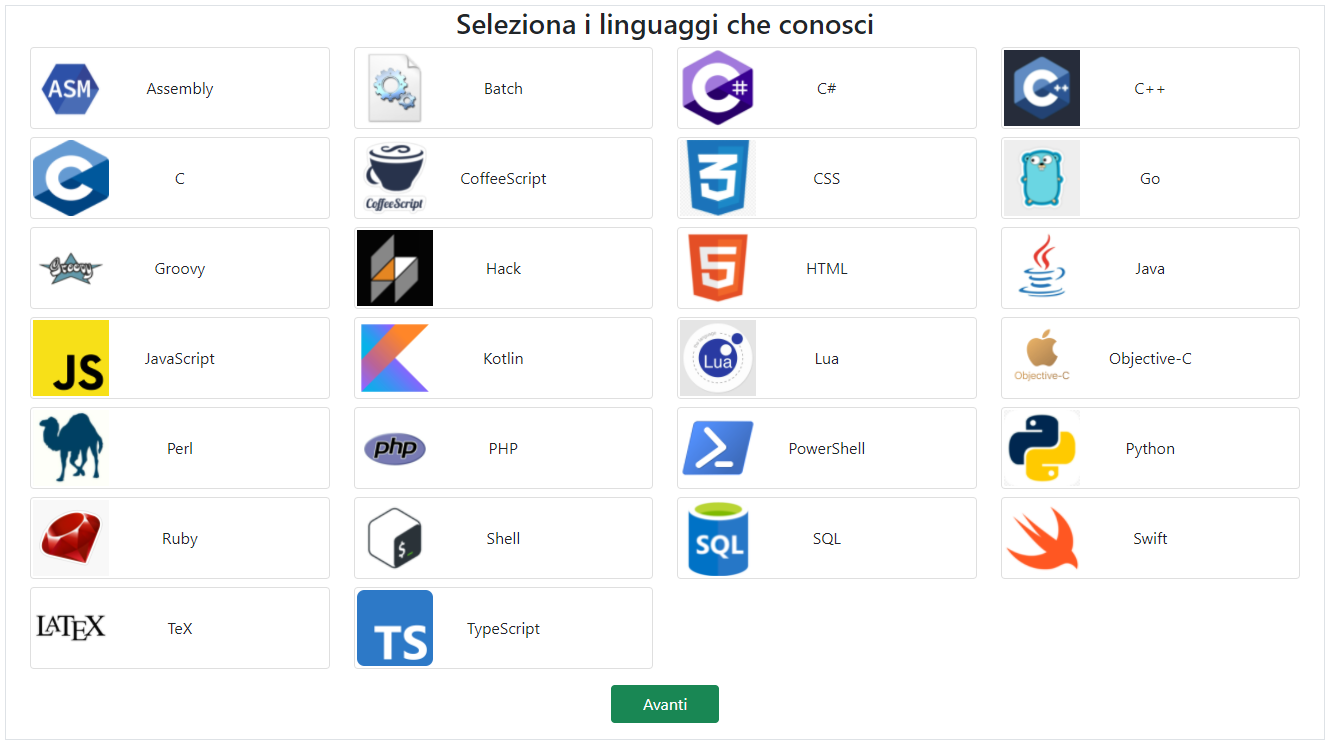
\includegraphics[width=\textwidth]{capitoli/images/linguaggi_padroneggiati.png}
    \caption{Form per l'inserimento dei Linguaggi padroneggiati dall'utente}
    \label{fig:linguaggi_padroneggiati}
\end{figure}
\begin{figure}[!htb]
    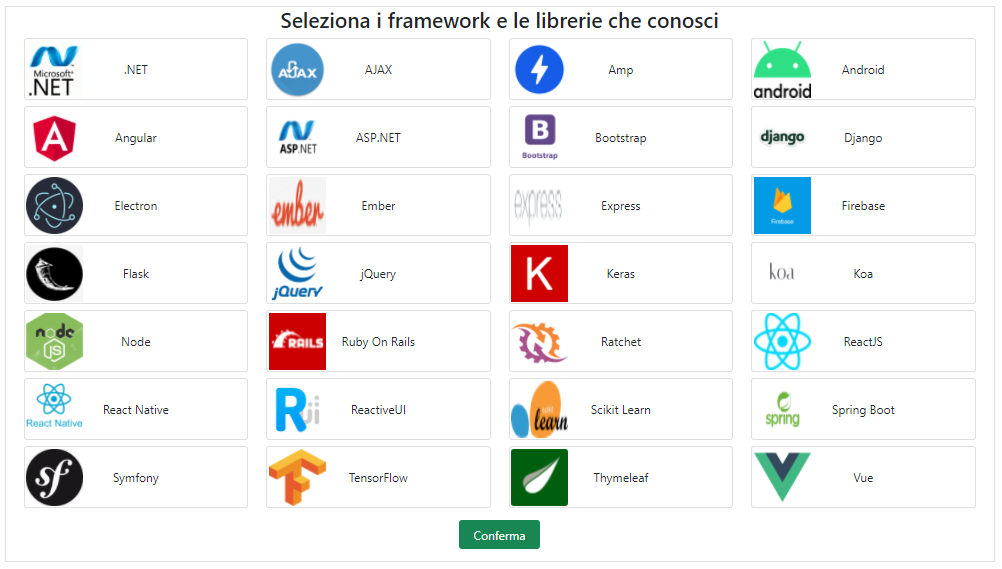
\includegraphics[width=\textwidth]{capitoli/images/frameworks_padroneggiati.png}
    \caption{Form per l'inserimento dei Frameworks e delle Librerie padroneggiate dall'utente}
    \label{fig:frameworks_padroneggiati}
\end{figure}
\\È possibile evitare che l'utente debba inserire manualmente le tecnologie che conosce, dandogli la possibilità di effettuare il Log In con \emph{GitHub} e chiedendogli di concedere l'autorizzazione alla lettura delle sue Repositories pubbliche e private. In questo modo è possibile prelevare i dati relativi alle tecnologie utilizzate nelle sue Repositories. A tal proposito è necessario fare due precisazioni:
\begin{itemize}
    \item In primo luogo ottenere le tecnologie utilizzate nella Repositories significa ottenere i Linguaggi, i Frameworks e le Librerie. I Linguaggi sono facilmente ottenibili grazie alle \emph{API} pubbliche messe a disposizione da \emph{GitHub} (un semplice modulo che effettua tale tipo di lavoro è stato facilmente implementato), mentre per quanto riguarda i Frameworks e le Librerie ci si affiderà ai tag delle Repositories (che non sempre contengono questo tipo di informazioni) e verranno utilizzate opportune tecniche per ricondurre il nome del tag al nome del Framework o della Libreria corrispondente, eventualmente andando ad utilizzare tecniche simili o del tutto equivalenti a quelle di \emph{NLP} presentate nel precedente capitolo.
    \item Il fatto che una determinata tecnologia sia presente in una Repository di cui l'utente risulta essere contributor, non significa necessariamente che l'utente padroneggi quella tecnologia; per tale ragione è opportuno che le tecnologie prelevate da \emph{GitHub} vengano proposte all'utente e che gli venga, dunque, data la possibilità di modificarle opportunamente.
\end{itemize}
Giunti a questo punto, la piattaforma suggerisce all'utente un insieme di Linguaggi, Frameworks e Librerie consigliati utilizzando le metodologie trattate nel capitolo precedente, come illustrato nella figura \ref{fig:tecnologie_suggerite}.
\begin{figure}[!htb]
    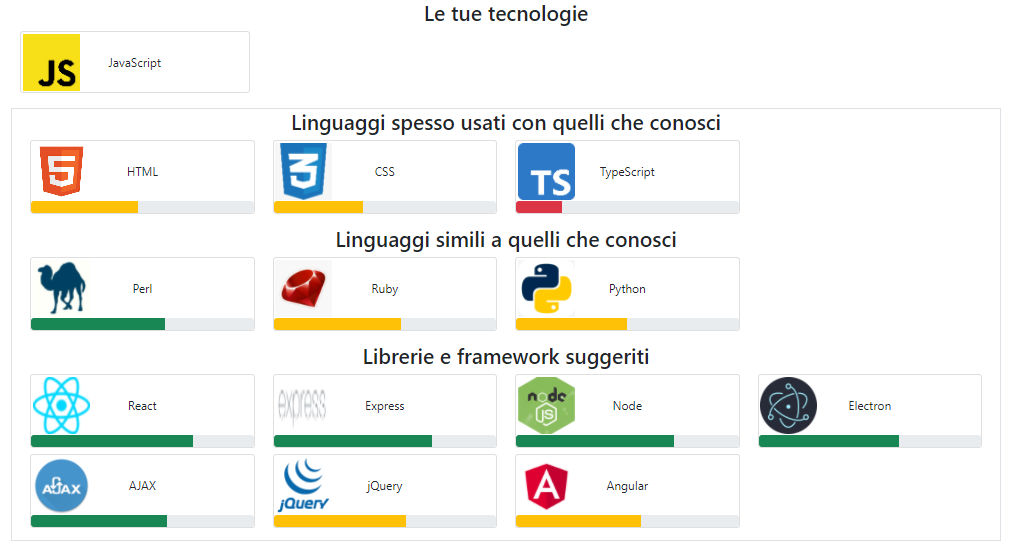
\includegraphics[width=\textwidth]{capitoli/images/tecnologie_suggerite.png}
    \caption{Risultato dell'Algoritmo che suggerisce Tecnologie Software}
    \label{fig:tecnologie_suggerite}
\end{figure}
\\L'utente può scegliere una o più tecnologie da imparare e la piattaforma provvederà a suggerirgli un insieme di utenti con cui iniziare una collaborazione mediante un algoritmo di Intelligenza Artificiale di cui è stato fornito un accenno di progettazione nel capitolo precedente. Due utenti si mettono in contatto tramite una richiesta di collaborazione che potrà essere effettuata solo se l’utente destinatario della richiesta padroneggia almeno una tecnologia che l’utente mittente vuole imparare e vuole imparare almeno una tecnologia padroneggiata dall’utente mittente. Se l’utente destinatario accetterà la richiesta, si creerà una collaborazione tra i due utenti; a questo punto la piattaforma deve fornire un insieme di strumenti che consentono ai due utenti di collaborare in maniera agevole ed efficiente. 
Di seguito verranno proposte e descritte diverse funzionalità:
\begin{itemize}
    \item Dovrebbe essere previsto un sistema di chat immediato che consenta agli utenti di comunicare in tempo reale per accordarsi sulle sessioni di "apprendimento"
    \item Le sessioni di apprendimento dovrebbero avvenire tramite lezioni in tempo reale, svolte mediante chiamate o videochiamate, in cui sia possibile condividere lo schermo per far sì che l’utente che insegna possa mostrare in tempo reale il codice che scrive e l’esecuzione dello stesso. Tali lezioni dovrebbero essere schedulate e la piattaforma dovrebbe tenere traccia dello schedule stesso mediante un calendario, che possa essere usato sia per tracciare lo schedule delle lezioni, che per aggiungerne di nuove. Un utente può aggiungere una lezione in cui lui sarà insegnante, potrà scegliere l’allievo e la tecnologia da insegnare e la lezione aggiunta verrà subito mostrata sul calendario dell'utente allievo. (figura \ref{fig:calendario}).
    \begin{figure}[!ht]
        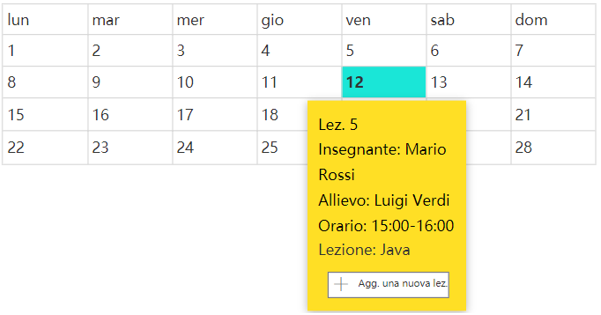
\includegraphics[width=\textwidth]{capitoli/images/calendario.png}
        \caption{Mockup del calendario che tiene traccia degli schedule delle lezioni}
        \label{fig:calendario}
    \end{figure}
    \item Il miglior modo per imparare è "provare sul campo", quindi dopo le sessioni di apprendimento è necessario che l’utente che sta imparando provi praticamente quanto ha appreso durante le lezioni. A tale scopo la piattaforma deve mettere a disposizione un sistema di assegnamento di task tramite il quale l’utente che sta insegnando può assegnare uno o più task all’utente che sta imparando. Il tutto potrebbe essere semplificato tramite un’integrazione con \emph{GitHub}, in modo tale che la piattaforma tenga traccia dei task (testo dell’esercizio), di un eventuale schedule dei task (tramite un calendario) e del link alla Repository di \emph{GitHub} contenente una proposta di soluzione svolta dall’utente che sta imparando, che verrà poi corretta dall’utente che insegna.
\end{itemize}
È importante sottolineare che i ruoli di "utente che insegna" e di "utente che impara" sono assolutamente dinamici in quanto nell’ambito di diversi meeting questi due ruoli potrebbero invertirsi (idealmente vi sarà un numero di meeting in cui l’utente A è insegnante e B è allievo, uguale al numero di meeting in cui l’utente A è allievo e B è insegnante). 
\section{Architettura del sistema} %\label{1sec:scopo}
La piattaforma \textsc{Code4Code} si concretizza in una \emph{WebApp} fruibile mediante un semplice Web Browser. Vi è un \emph{Web Server} scritto in \emph{Java} che serve le richieste del Client mediante delle \emph{REST API}. Durante l'utilizzo della piattaforma si interagisce con tre ulteriori Server:
\begin{itemize}
    \item Il primo Server, scritto in \emph{Python}, fornisce i risultati del modulo di Intelligenza Artificiale che suggerisce Frameworks e Librerie all'utente.  
    \item Il secondo Server è quello di \emph{Mattermost} \cite{mattermost}, strumento pensato per risolvere il problema delle chiamate e delle videochiamate con condivisione schermo. \emph{Mattermost} è una piattaforma \emph{open source} e \emph{self-hosted} a sé stante, ideata per la collaborazione nell'ambito di un'organizzazione e che fornisce servizi di chat in tempo reale con tanto di condivisione di file, chiamate, videochiamate, creazione di canali di comunicazione, funzionalità di condivisione schermo, il tutto accessibile mediante Web Browser come il resto delle funzionalità della piattaforma \textsc{Code4Code}. Dal momento che \emph{Mattermost} è \emph{open source}, è possibile ricompilare i sorgenti per modificare sia il \emph{Front-End} che il \emph{Back-End} della piattaforma al fine di adattarla ulteriormente al contesto di utilizzo evitando gli utilizzi impropri e decontestualizzati da parte dell'utente.
    \item Il terzo Server è il \emph{DataBase Server} che mediante un apposito \emph{DBMS} gestisce le entità persistenti della piattaforma.
\end{itemize} 
\begin{figure}[!htb]
    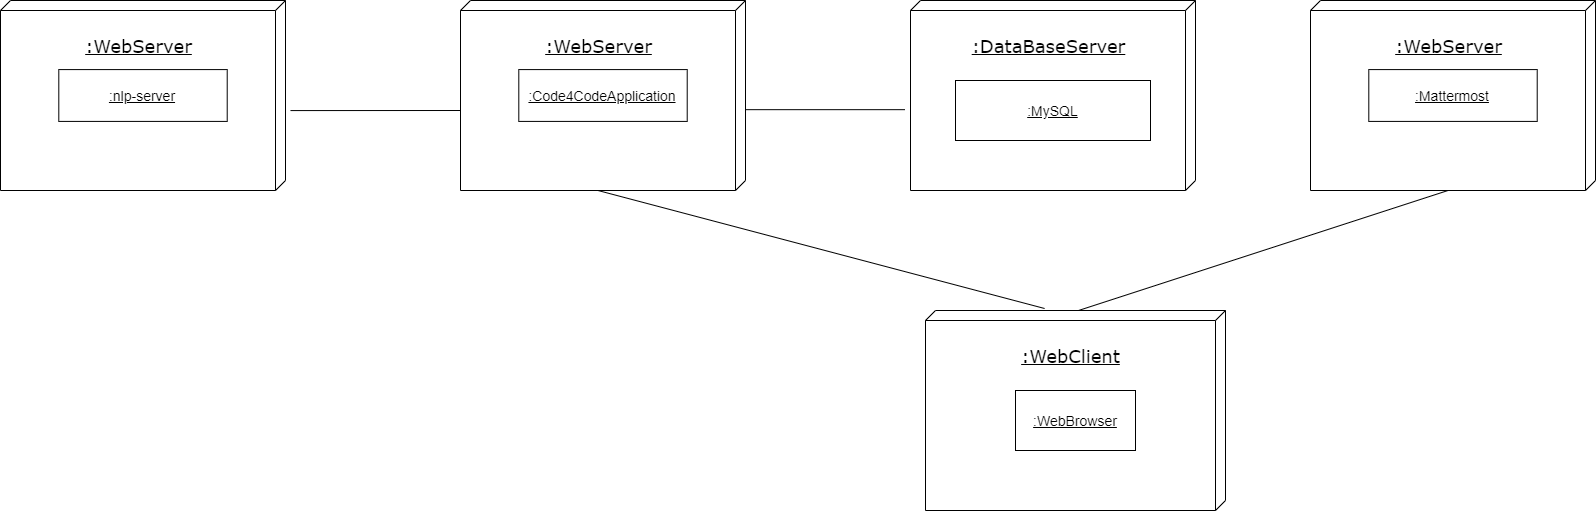
\includegraphics[width=\textwidth, height=6cm]{capitoli/images/progettazione_c4c.png}
    \caption{Architettura della piattaforma \textsc{Code4Code}}
    \label{fig:progettazione_c4c}
\end{figure}
\section{Framework utilizzati}
Per la realizzazione della piattaforma \textsc{Code4Code} sono stati impiegati vari Frameworks e Librerie. 
\begin{itemize}
    \item Per il \emph{Web Server} in \emph{Java} è stato utilizzato \emph{Spring} che ha reso agevole e veloce lo sviluppo delle \emph{REST API} implementate. Inoltre è stato utilizzato il motore di template \emph{Thymeleaf} per uno sviluppo moderno delle pagine \emph{HTML}, la cui parte grafica è stata facilmente curata grazie al Framework \emph{Bootstrap}.
    \item Per la parte di \emph{Natural Language Processing} in \emph{Python} è stata usata la Libreria \emph{Gensim} che ha fornito un'implementazione dell'algoritmo \emph{Word2Vec} per l'addestramento della Rete Neurale.
    \item Per le \emph{Association Rules}, utilizzate per il suggerimento dei Linguaggi, è stata utilizzata la Libreria \emph{Apyori} grazie alla quale è possibile usufruire dell'implementazione dell'algoritmo \emph{Apriori} per la generazione delle \emph{Association Rules}.
    \item Per il \emph{Web Server} in \emph{Python} è stato utilizzato \emph{Flask}, che ha consentito di configurare il Server in maniera agevole con poche righe di codice.   
\end{itemize}
\newpage

\chapter{Conclusioni} %\label{1cap:spinta_laterale}
% [titolo ridotto se non ci dovesse stare] {titolo completo}
%


\begin{citazione}
	BREVE SPIEGAZIONE CONTENUTO CAPITOLO
\end{citazione}

\newpage


\backmatter
%*******************************************************
% Bibliografia
%*******************************************************
\cleardoublepage
\phantomsection
\addcontentsline{toc}{chapter}{\bibname}
\nocite{*}
\bibliographystyle{unsrt}
\bibliography{bibliografia}

\vspace{2.5cm}
\begin{Large}Siti Web consultati\end{Large}
\begin{itemize}
    \item Wikipedia -- \url{www.wikipedia.org}
    \item Lorenzo Govoni -- \url{www.lorenzogovoni.com}
    \item Seart GitHub Search -- \url{https://seart-ghs.si.usi.ch/}
\end{itemize}


\begin{titlepage}

\nonumber
\null \vspace {\stretch{1}}
	\begin{flushright}
%	\begin{verse}
\textit{"Perché il miglior risultato si ottiene quando ogni componente del gruppo farà ciò che è meglio per sé... e per il gruppo..."\\- John Nash} \\[5mm]
%	\end{verse}
	\end{flushright}



\end{titlepage}
\end{document}
